%% section_text.tex -- follow-up paper Section 2 (Census)
\section{Scale-invariant census across Hristov 2024}
\label{sec:census}

The equations of motion for the equal-mass three-body problem with $G = m_i = 1$
admit the one-parameter scaling group $r \to \alpha r$, $t \to \alpha^{3/2} t$.
The two scale invariants of a bound orbit at fixed $L = 0$ collapse to a
single number, $T^{\star} \equiv T\,|E|^{3/2}$, which together with $E$
characterises the orbit up to overall rescaling. Because our four orbits live
on the Euler velocity section where $L_z = 0$ identically
(Section~\ref{sec:klein}), and because the Hristov 2024 catalogue is also a
zero-angular-momentum set, both live on the same $(E, T^{\star})$ plane.

We computed $(E, T^{\star})$ for all 24\,582 Hristov 2024 entries from their
catalog initial conditions and periods (compute time $<1\,\mathrm{s}$ on CPU).
Figure~\ref{fig:census-scatter} overlays the result with our four orbits; the
Hristov ensemble forms a dense density that extends to $E \approx -15$, while
A, B, C, D sit in the sparse high-energy region at $E \approx -1$ to $-2$.
Figure~\ref{fig:census-density} shows the 1-D density of $T^{\star}$ across
the full catalog: A at $T^{\star} = 36.9$ lies well to the left of the
distribution peak (roughly $T^{\star} \sim 70$-$80$), while C and D lie near
the peak (consistent with their identification as Hristov 2025 catalog
entries \#0006 and \#0011). B sits at $T^{\star} = 64.65$, differing from C
by $\Delta T^{\star}/T^{\star} \approx 10^{-4}$ but with distinct energy:
a near-coincidence in one invariant without coincidence in the other, implying
a genuinely different bifurcation branch of the same topological class.

\begin{figure}[t]
\centering
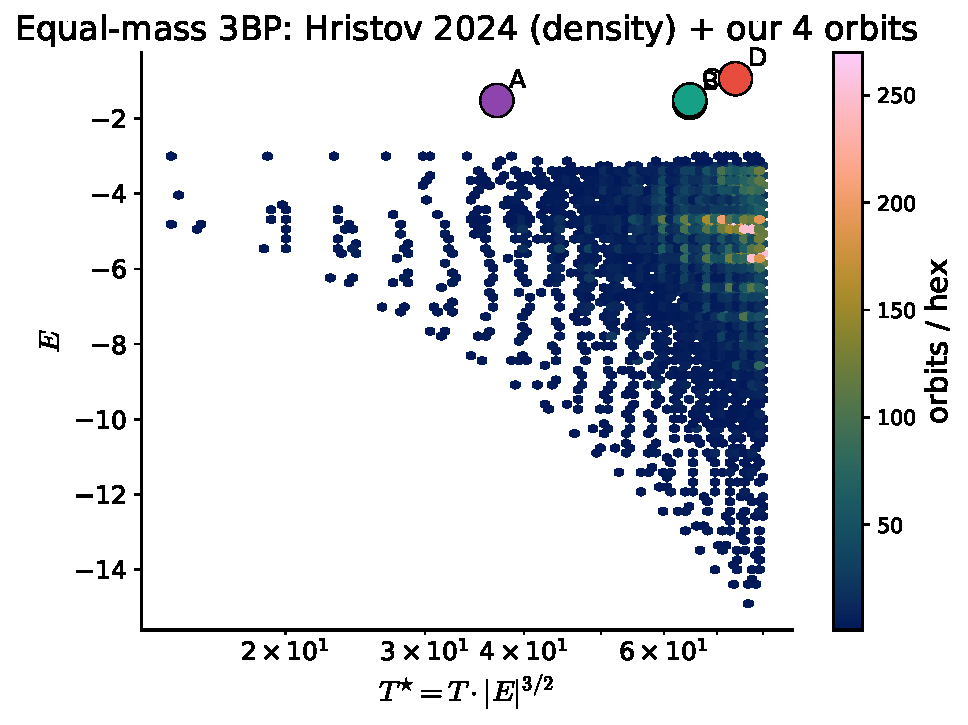
\includegraphics[width=0.95\linewidth]{figures/census_scatter_paper.pdf}
\caption{$(E, T^{\star})$ scatter of 24\,582 Hristov 2024 periodic orbits,
rendered as a hex density (viridis-family colormap). Our four orbits A, B,
C, D overlay the density at their measured $(E, T^{\star})$ values. All four
sit in the sparse high-$E$ region, above the peak of the Hristov ensemble.}
\label{fig:census-scatter}
\end{figure}

\begin{figure}[t]
\centering
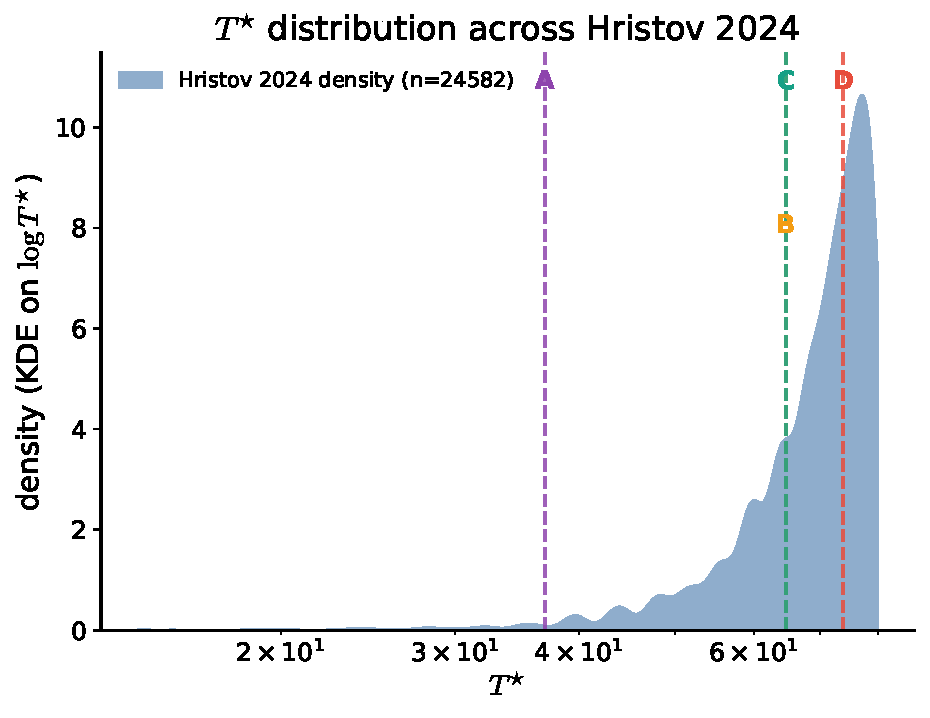
\includegraphics[width=0.95\linewidth]{figures/census_density_paper.pdf}
\caption{KDE of $T^{\star}$ across the full Hristov 2024 catalogue.
Dashed vertical lines mark our four orbits. Orbit A is well outside the
distribution peak; C and D lie at the peak.}
\label{fig:census-density}
\end{figure}

\begin{figure}[t]
\centering
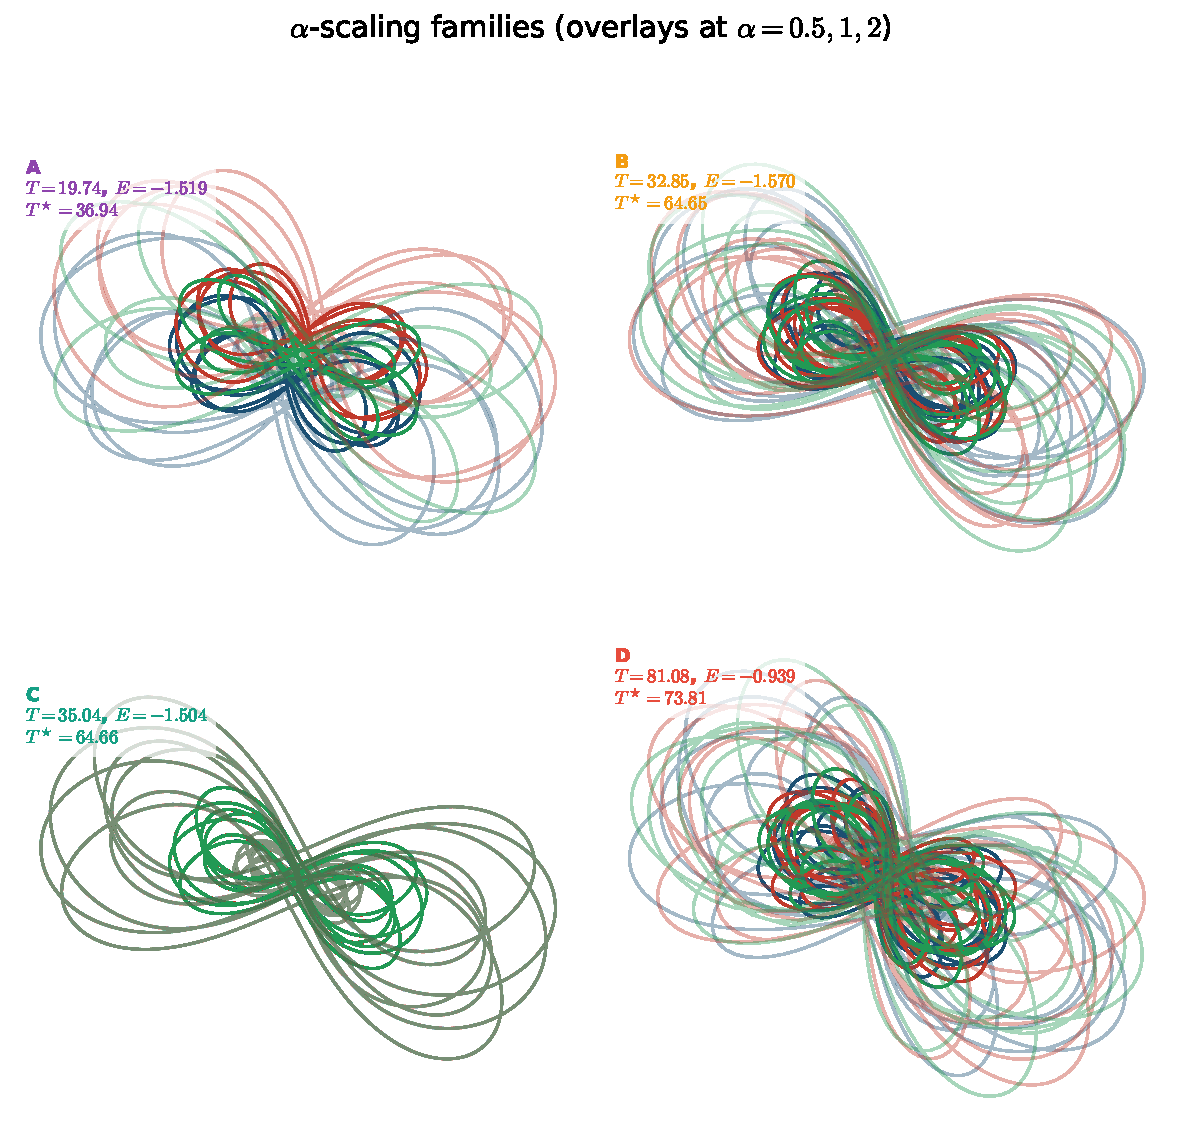
\includegraphics[width=0.9\linewidth]{figures/scaling_families_paper.pdf}
\caption{$\alpha$-scaling families for A, B, C, D. Overlays at $\alpha = 0.5, 1, 2$
demonstrate that topology is invariant under rescaling while linear size and
period change. In panel C all three bodies trace a single curve (up to a
one-third-period shift), a manifestation of the figure-8-type symmetry of the
Hristov 2025 \#0006 family.}
\label{fig:scaling-families}
\end{figure}
